\documentclass[12pt]{article}
\usepackage[utf8]{inputenc}
\setlength{\parindent}{0pt}	% set zeno indent at the beginning of each paragraph

\usepackage{graphicx}	% for using image in the doc
\graphicspath{ {./images/} }	% for using image in the doc

\usepackage{makecell}    % for using table
\usepackage{multirow}    % for using table
\usepackage{amsmath}

\usepackage{url}

\newcommand{\rotcelltwo}[1]{%
  \rotatebox[origin=c]{90}{ #1 }%
  \centering
}

\title{Mars Economy Project Whitepaper}
\author{
  The Mars Economy Community\\
  fgrey650\\
  jet-jelly\\
  Vasco-d-Gama\\
  ollo\\
}

\date{May 2021}

\begin{document}

\maketitle


% ---------------------------------- Abstract ------------------------------------
\begin{abstract}
This whitepaper contains a technical description of the Mars Economy project principles, architecture, smart contracts, token distribution and governance. Mars Economy is a decentralized platform that attracts public interest and financial resources to projects aimed at future colonization of Mars. The Mars Economy project will have 2 phases: the Prediction market phase and the Martian financial ecosystem phase. The Mars Economy project consists of a set of project specific markets where users can stake on important events on the way to the colonization of Mars. Settlement of the prediction markets will be done by a group of oracles or, if the oracles cannot come to consensus, by voting of all the \$DMT token holders. The Mars Economy project is a Decentralized Autonomous Organization (DAO) governed by the community of \$DMT token holders.
\end{abstract}


% ---------------------------------- About the authors ------------------------------------
\section{About the authors}

This document is prepared and maintained by a team of contributors known as The Mars Economy Community. The Mars Economy project is governed by a decentralized autonomous organization (DAO) where every member has rights to contribute and participate in decision making. To emphasize the community-driven nature of the project, we do not personalize the authors but list their GitHub nicknames.

% ----------------------------- Project overview -----------------------------------------
\section{Project overview}

Mars Economy is a decentralized platform that attracts public interest and financial resources to projects aimed at future colonization of Mars. In the beginning, the Mars Economy project will act as a prediction market allowing users to stake on the outcomes connected with the colonization of Mars. The Mars Economy project will also facilitate mostly promising projects by rewarding them with native \$DMT tokens.

In the future \$DMT tokens should become a basis for a decentralized open financial ecosystem on Mars.
 
% ----------------------------- Project phases -----------------------------------------
\section{Project phases}

The Mars Economy project will have 2 phases:
\begin{itemize}
    \item{The Prediction market phase} will be the initial phase, during which the project will implement prediction market contracts allowing people to stake on the outcomes related to the future colonization of Mars. During this phase also the initial distribution and market creation for \$DMT tokens will be accomplished. \$DMT tokens in this phase will serve as a basis for the sustainable oracle system and as a voting token for the decentralized governance.
    \item{The Martian financial ecosystem phase} will start with the first achievements in the colonization of Mars. In this phase \$DMT tokens will become an exchange medium for financial transactions both on Mars and between Mars and Earth.
\end{itemize}

% ------------------------------ Prediction market operations ----------------------------------------
\section{Prediction market operations}

\subsection{Prediction markets structure}
The Mars Economy project consists of a set of project specific markets. The most promising projects, elected by the Mars Economy decentralized governance, will be allowed to open specific staking on the platform. For each of these projects a separate prediction market will be created. Unlike e.g. Augur, new prediction market creation decisions can be only taken by voting of all \$DMT token holders.

The markets use 3-level grouping: 
\begin{itemize}
\item{Level 1 - Phases.} Examples are: Crossing the frontier; Discover the red planet; A new home.
\item{Level 2 - Milestones.} Examples are: First Orbital Flight of spacecraft fit for Mars logistics; First crew headed to Mars.
\item{Level 3 - Predictions.} Examples are: Achieved by XX.XX.20XX (yes / no)? Private Company or NASA SLS? Which Agency or Nation will be the first ? What is the crew size ?
\end{itemize}

All prediction markets operate identically based on the same smart contracts code.

The basic attributes of all prediction markets are:
\begin{itemize}
\item A complete set of possible outcomes.
\item A settlement date.
\item Time and pool share limits.
\end{itemize}

Decisions about the winning outcomes are taken at the settlement date by a group of oracles or by governance under control of a separate Settlement smart contract.

\subsection{The role of \$DMT tokens in the prediction market phase}

\$DMT tokens play two major roles in the Mars Economy project in the prediction market phase:
\begin{itemize}
\item{Basis for the Mars Economy oracle system.} All parties that are allowed by the Mars Economy decentralized governance to act as oracles, must stake 100,000 \$DMT tokens. The staked tokens are locked in the Settlement smart contract until the date of settlement of a certain prediction market.
\item{Voting token for decentralized governance.} Holders of \$DMT tokens will be able to submit governance proposals and vote for them, e.g.:
	\begin{itemize}
	\item Add a project specific market.
	\item Add / remove an oracle.
	\item Change fees.
	\item Setup a future emission control smart contract.
	\end{itemize}
\end{itemize}

\subsection{Creation of a prediction market}
A new prediction market is created by governance decision. When the decision is approved, a new instance of the prediction market smart contract is automatically deployed in the blockchain using the Factory smart contract.

\subsection{Shares of outcomes}
Every Mars Economy prediction market has shares of outcomes tokens that can be either bought directly from the Mars Economy prediction market contracts or traded on an external market. Every share corresponds to one of the possible outcomes for a given market. At the date of settlement the shares for the true outcome will be accepted by the Mars Economy prediction market smart contract at the \textbf{settlement price} (see details below), alternative shares will not be accepted and therefore will have no value.

The initial shares distribution will be performed by the Mars Economy smart contract. The price of shares will not be fixed, but will grow gradually over time. This will incentivize users to buy the shares early and also will provide some interest on assets locked in the smart contract. 

Provided that:
\begin{itemize}
    \item start\_price (SP) is a starting share price;
    \item end\_price (EP) is an ending share price;
    \item prediction\_time\_start (PTS) is a time moment when a market has started operation;
    \item prediction\_time\_end (PTE) is a time moment when staking will be closed;
    \item current\_time (CT) is now.
\end{itemize}

Then

\[ share\_price = \frac{(EP - SP)(CT - PTS)}{PTE - PTS} + SP\]

If, for example, the annual price increase rate is 50\% and the start\_price is 1 BUSD, then the end\_price for a 2-year prediction will be 3 BUSD, for a 10-year prediction - 15 BUSD. The price will be recalculated every week. If at some point of time the share\_price of some outcome will exceed an estimated reward for a given market, the smart contract will temporarily suspend staking on this outcome until the reward will grow to fit the price. This will protect early stakers from loosing their profits as early staker rewards can never become lower than later staker rewards.

All the collected amount will be locked in the Mars Economy prediction market smart contract until the prediction date. When a winning outcome will be settled, the collected amount will be distributed among the winning shareholders proportionally by returning their shares to the smart contract and burning them.

To prevent staking on events when some outcome becomes obvious earlier than the prediction date, the prediction\_time\_end limit (defined for each prediction market) can be set earlier than the prediction date. It will be also possible to shift this limit by governance, but only back in time - to protect profits of existing stakers.

\subsection{Settlement price of the shares}
The settlement price of the winning shares will include the initial amount of BUSD collected minus the amount of fees paid to oracles, minus the protocol fee:

\[ settlement\_price = \frac{total\_BUSD\_collected - oracle\_fees\_paid - protocol\_fee}{number\_of\_shares\_won} \]

\subsection{Fees}
The Mars Economy protocol will charge fees for every purchase of shares. When a certain number of shares is bought, 0.3\% will be taken: 0.2\% will go to the oracles, 0.1\% will be the protocol fee. Fee values may be changed by governance.

\subsection{Settlement smart contract, oracle staking}
A list of approved oracles is stored in the settlement smart contract and may be changed by governance. Each oracle is identified by a wallet id from which \$DMT tokens must be staked. The prediction markets operation and sale of shares of outcomes is allowed only when at least one oracle has staked 100,000 \$DMT tokens on the contract. Only approved (by governance) oracles are eligible for staking. 

Oracles may withdraw their stakes unless:
\begin{enumerate}
\item It is the last oracle in the list. The last oracle is not allowed to withdraw his stake until some other oracle makes a new stake.
\item All the staked tokens are blocked by the settlement smart contract when a settlement procedure starts on any prediction market until the end of the settlement procedure.
\end{enumerate}

\subsection{Settlement protocol}
When the settlement date for a given market comes, all the oracles must report the true outcome within 24 hours. All oracles have equal weights when reporting.

If 100\% of the oracles are in consensus, the winning outcome is defined as a tentative outcome and the dispute phase starts.

The dispute phase lasts for 7 days during which any \$DMT tokens holder can stake 20,000 \$DMT tokens to start a dispute. If a dispute is started, the voting phase starts.

If less than 100\% of the oracles vote for one outcome or in case of a dispute, the voting phase starts, during which all \$DMT token holders may vote for outcomes. Corresponding governance decisions are created automatically by the Settlement smart contract in these cases:
\begin{enumerate}
\item Within a dispute start transaction, or
\item Initiated by anybody using the \textbf{startVoting} public method in the Settlement smart contract (this method becomes available after 24 hours from the settlement date if there is no consensus).
\end{enumerate}

Every \$DMT token holder will have the number of votes equal to the number of \$DMT tokens in possession. The voting phase will last for 7 days.

If the quorum threshold is passed for the voting phase, the voting decision is considered final. If the quorum threshold is not passed after 7 days, the voting phase is repeated for another 7 days with the quorum threshold decreased by 50\%. This procedure loops until the quorum is reached. The initial quorum threshold will be 10\% and may be changed by governance.

If nobody starts a dispute within the dispute phase, the decision is considered final automatically.

\subsection{Incentives and penalties}
Oracles are incentivized for staking their \$DMT tokens with oracle fees (0.2\%) from every buying transaction on the platform. The fees are sent to the oracles after the final settlement. Only the oracles whose opinions conform with the final decision will get the fees. The total amount of fees will be divided between the conforming oracles equally. If no oracles voted successfully, the whole amount of oracle fees will be used as an additional protocol fee.

The staked \$DMT tokens will be returned only after the settlement procedure. Only oracles that voted for an outcome that was finally decided true will get their \$DMT tokens back. Oracles that voted wrong or failed to vote within the defined time window will not get the tokens back. 20\% of these forfeited tokens will be burnt, other 80\% will be distributed equally among the successful oracles. If no oracles voted successfully, all 100\% of the forfeited tokens will be burnt.

Oracles that voted wrong or failed to vote within the defined time window are automatically removed from the list of approved oracles. This is done in the same transaction with finalization of the voting phase for a settlement decision.

A \$DMT token holder that staked his tokens to start a dispute will get his tokens back only if the dispute will change the initial tentative outcome. Otherwise, 20\% of these forfeited tokens will be burnt, other 80\% will be distributed equally among the successful oracles.

\subsection{Protocol fee}
The protocol fee will be initially set to 0.1\% from every purchased share of outcomes. This fee may be claimed at any time by the owner of a predefined wallet id.

The protocol fee receiver's wallet id and the protocol fee level may be changed by governance.


% ------------------------------- Distribution of \$DMT tokens ---------------------------------------
\section{Distribution of \$DMT tokens}

\subsection{Initial distribution}
The total token supply for the prediction market phase is 1,000,000,000 \$DMT tokens distributed in 5 pools:
\begin{itemize}
\item{Core team pool (100M \$DMT)} - distributed among the core team.
\item{Strategic investors pool (100M \$DMT)} - for investors of the first round.
\item{Ecosystem pool (350M \$DMT)} - to attract strategic partners:
	\begin{itemize}
	\item{300M \$DMT} for key strategic partners (SpaceX, BlueOrigin, Moonx, and so on).
	\item{50M \$DMT} to promote individuals and the broader community of space enthusiasts to be actively involved in the promotion of Mars exploration related activities.
	\end{itemize}
\item{Fundraising pool (50M \$DMT).}
\item{Common pool (400M \$DMT)} - for future ecosystem/users.
\end{itemize}

Tokens from the core team pool, the strategic investors pool, the ecosystem pool and the fundraising pool are distributed based on ongoing voting proposals.

\$DMT tokens distributed among the core team will be \textbf{subject to lock-in} for 2 years from the project launch. During the lock-in period the core team members will be eligible to vote for governance proposals and create them, but the ownership of tokens may not be transferred.

\subsubsection{Ecosystem pool distribution}
Ecosystem pool tokens will be gradually distributed among representatives (preferably companies) advancing the colonization of Mars. The actual distribution will be carried out by means of smart contract voting by current \$DMT governance token holders.

\subsubsection{Common pool distribution}
Common pool will be made gradually available for purchase via exchanges and DEXes, also by means of IEOs and IDOs.

% ---------------------------- Governance ------------------------------------------
\section{Governance}

\subsection{Basic principles}
The Mars Economy project is a Decentralized Autonomous Organization (DAO) governed by the community of \$DMT token holders. No other person or entity has reserved rights to influence the project parameters, including the smart contracts owner.

The Mars Economy project governance exists in 2 forms:
\begin{itemize}
\item{On-chain governance} is performed under control of the governance smart contract.
\item{Off-chain governance} is performed using the Snapshot software.
\end{itemize}

\subsection{On-chain governance}
When on-chain governance is applied, every action, including proposal submissions and voting, is a blockchain transaction. The drawback is that all these actions will require network fees (gas) to be paid by the participants. The outcomes are: all votes are immutably and reliably stored on the blockchain; approved decisions may be automatically fulfilled by the governance smart contract.

To submit a proposal, a user must stake 100,000 \$DMT tokens. These tokens will be locked in the governance contract until the end of voting on the proposal. The staked tokens will be returned only if the proposal is approved or quorum not reached. Otherwise, the staked tokens will be burnt.

Voting for each proposal lasts for 7 days. Every \$DMT token holder may vote for any proposal. The number of votes equals the number of tokens in possession. To vote, a user sends his \$DMT tokens to be temporarily locked in the governance contract to prevent double voting. The tokens are returned when the voting ends.

To approve a decision, a certain share of \$DMT token holders must vote according to the quorum threshold. The initial quorum threshold is 10\% and may be changed by governance. 

Therefore, we use on-chain governance only for decisions that can be done fully automatically:
\begin{itemize}
\item Prediction outcome decisions during the dispute and voting phases.
\item Create a new prediction market.
\item Shift an ending time for predictions back in time for a given prediction market.
\item Change oracles list.
\item Transfer tokens from the core team pool, the strategic investors pool, the ecosystem pool or the fundraising pool to a specific wallet.
\item Change the oracle fee level.
\item Change the protocol fee level.
\item Change the receiver of the protocol fee.
\item Change the period for oracles to make decisions.
\item Change the length of the dispute phase.
\item Change the length of the voting phase.
\item Change the quorum threshold.
\item Change the amount of tokens staked by an oracle.
\item Change the amount of tokens staked to start a dispute.
\item Change the amount of tokens staked to submit a proposal.
\end{itemize}

\subsection{Off-chain governance}
Off-chain governance is used to discuss and vote for decisions that cannot be formalized within the governance smart contract. Examples of these decisions could be:
\begin{itemize}
\item Propose development of new features.
\item Preliminary voting before submitting an on-chain proposal.
\end{itemize}

Off-chain governance uses Snapshot as a voting platform. Only \$DMT token holders are eligible to vote. The off-chain decisions are advisory and are fulfilled by the core project team.
\pagebreak

% ---------------------------- Architecture ------------------------------------------
\section{Architecture}

\begin{figure}[h!]
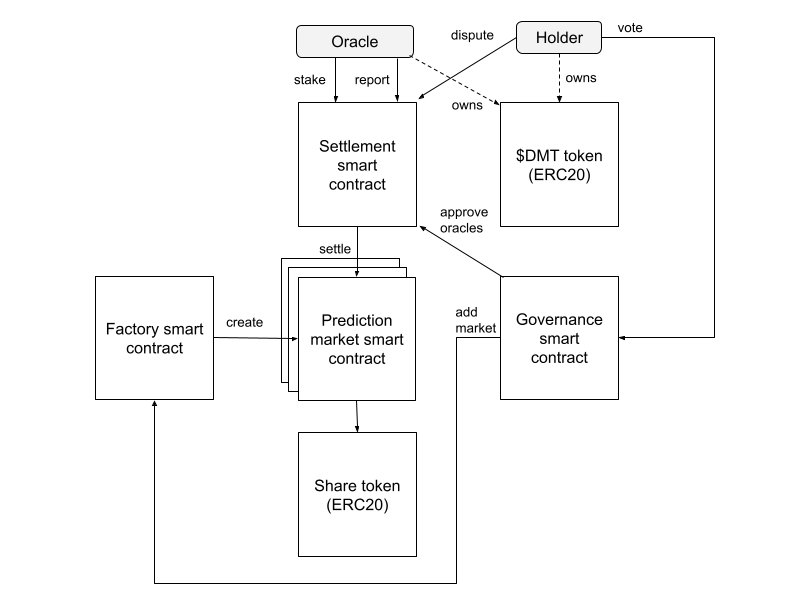
\includegraphics[scale=0.5]{Architecture}
\centering
\caption{Mars Economy smart contracts architecture}
\label{fig:architecture}
\end{figure}

\pagebreak
% ---------------------------------- Disclaimer ------------------------------------
\section*{Disclaimer}

The information provided in this paper does not constitute investment advice, financial advice, trading advice, or any other sort of advice and you should not treat any of the paper's content as such. By purchasing \$DMT, you agree that you are not purchasing a security or investment and you agree to hold the team harmless and not liable for any losses or taxes you may incur. You also agree that the team is presenting the token "as is" and is not required to provide any support or services. You should have no expectation of any form from \$DMT and its team. Although \$DMT is an EXPERIMENTAL token for social experiment and not a digital currency. Always make sure that you are in compliance with your local laws and regulations before you make any purchase.

\end{document}
